
%%% PREAMBLE 
\documentclass[9.5pt,lineno]{RandlettLab_elife}
\nolinenumbers
\usepackage{setspace}
\usepackage{lipsum} % Required to insert dummy text
\usepackage{listings}
\usepackage[version=4]{mhchem}
\usepackage{siunitx}
\usepackage{gensymb}
\DeclareSIUnit\Molar{M}
\usepackage{cancel}
\usepackage{xcolor}
\usepackage{textgreek}
\usepackage{soul} 
\usepackage{caption}
\definecolor{codegreen}{rgb}{0,0.6,0}
\definecolor{codegray}{rgb}{0.5,0.5,0.5}
\definecolor{codepurple}{rgb}{0.58,0,0.82}
\definecolor{backcolour}{rgb}{0.96,0.96,0.96}

\lstdefinestyle{mystyle}{
    backgroundcolor=\color{backcolour},   
    commentstyle=\color{codegreen},
    keywordstyle=\color{magenta},
    numberstyle=\tiny\color{codegray},
    stringstyle=\color{codepurple},
    breakatwhitespace=false,         
    breaklines=true,                 
    captionpos=b,                    
    keepspaces=true,                 
    numbers=left,                    
    numbersep=5pt,                  
    showspaces=false,                
    showstringspaces=false,
    showtabs=false,                  
    tabsize=2
}

\lstset{style=mystyle}
\tolerance=9999
\emergencystretch=10pt
\hyphenpenalty=1000000
\exhyphenpenalty=100
%%%%%%%%%%%%%%%%%%%%%%%%%%%%%%%%%%%%%%%%%%%%%%%%%%%%%%%%%%%%
%%% ARTICLE SETUP
%%%%%%%%%%%%%%%%%%%%%%%%%%%%%%%%%%%%%%%%%%%%%%%%%%%%%%%%%%%%
\title{A nocturnal increase in habituation learning performance is governed by Melatonin acting via the cooperative action of two MT1-type GPCRs. 
}

\author[1] 
{Dominique Baas}


\author[1, @] 
{Owen Randlett}


\affil[1]{
Laboratoire MeLiS, Université Claude Bernard Lyon 1 - CNRS UMR5284 - Inserm U1314, Faculté de Médecine et de Pharmacie, 8 avenue Rockefeller, 69008 Lyon, France
}


\affil[!]{equal contribution}

\affil[*]{equal contribution}


\affil[@]{correspondence: \href{mailto:owen.randlett@univ-lyon1.fr}{owen.randlett@univ-lyon1.fr}, ORCID: \href{https://orcid.org/0000-0003-0181-5239}{0000-0003-0181-5239}}

%%%%%%%%%%%%%%%%%%%%%%%%%%%%%%%%%%%%%%%%%%%%%%%%%%%%%%%%%%%%
%%% ARTICLE START
%%%%%%%%%%%%%%%%%%%%%%%%%%%%%%%%%%%%%%%%%%%%%%%%%%%%%%%%%%%%

\begin{document}

% \doublespacing
\maketitle

% \section{Disclosures}

% The authors have nothing to disclose.

\section{Keywords}

Melatonin, Melatonin Receptors, Habituation, Learning, Zebrafish, Larva, Sensorimotor Gating, Startle Response

% \section{Corresponding Author}
% Owen Randlett
% \\ Team ZeNeB: Zebrafish Neurogenetics and Behaviour
% \\ Laboratoire MeLiS, UCBL - CNRS UMR5284 - Inserm U1314, Institut NeuroMyoGène, 
% \\ Faculté de Médecine et de Pharmacie, 8 avenue Rockefeller, 69008 Lyon
% \\ \emph{email:} \href{mailto:owen.randlett@univ-lyon1.fr}{owen.randlett@univ-lyon1.fr}
% \\ \emph{ORCID:} \href{https://orcid.org/0000-0003-0181-5239}{0000-0003-0181-5239}


% \newpage
\begin{abstract}
  
Melatonin is a circadianly-regulated hormone that is produced by the pineal gland and the retina that has important roles not only in regulating sleep and circadian rhythms, but also other diverse physiological processes, including neuronal plasticity and learning. 
Melatonin is though to signal primarily through two G-protein coupled receptors, MT1 (Mtnr1a) and MT2 (Mtnr1b), which are expressed in the brain and other tissues.

\end{abstract}

\section{Introduction}

Melatonin is a circadianly-regulated hormone that is produced by the pineal gland and the retina that has important roles not only in regulating sleep and circadian rhythms, but also other diverse physiological processes, including neuronal plasticity and learning. 
Melatonin is though to signal primarily through two G-protein coupled receptors, MT1 (Mtnr1a) and MT2 (Mtnr1b), which are expressed in the brain and other tissues.


\section{Results}
\subsection{Melatonin induces bidirectional changes in visual habituation learning}

Through a high-throughput drug screen, we previously identified Melatonin as a potent modulator of habituation learning in larval zebrafish \citep{Lamire2023-he}. Based on this previous dataset, we concluded that Melatonin potently enhances habituation learning for the probability of executing an O-bend response to repeated dark-flash stimuli. Importantly, we found that Melatonin had little effect on the habituation of the magnitude of the O-bend response, which is governed by a distinct plasticity mechanisms \citep{Randlett2019-fj}, and Melatonin did not affect the response of the animals to acoutsic or optomotor stimuli \citep{Lamire2023-he}. This demonstrates that Melatonin does not have a generalized effect on sensory processing or motor output (e.g. by simply inducing sleep \citealp{Hill2026, Gandhi2015_NEURON}). 

We have extended these analyses using a larger dataset, and confirmed that acute exposure to \SI{1}{\micro\Molar} Melatonin potently enhances habituation learning for the probability of response (\autoref{fig:1}A). Further, a significant enhancement of habituation was also observed for the response Latency, which increases by >100 msec over habituation training (\autoref{fig:1}B). In both of these measures of behaviour, the response of the larvae to the acoustic stimuli is indistinguishable ("Acoustic Response": \autoref{fig:1}Ai,v, Bi,v)). The response to the first 3 dark-flash stimuli are not dramatically altered by the treatment ("Naive Response": \autoref{fig:1}Aii, Bii), but the effect is pronounced during the remaining 57 flashes of the first training block ("Block 1" \autoref{fig:1}Aii, Bii), the 180 flashes in the subsequent 3 training blocks ("Trained Response": \autoref{fig:1}Aiii, Biii), and the re-test block 5 hours after the last training session ("Block 5": \autoref{fig:1}Avi, Bvi). From these data we can conclude that Melatonin potentiates habituation learning for these two components of behaviour. 

This larger dataset now also more clearly reveals the effects of Melatonin on habituation of behavioural components related to the magnitude of the O-bend response. While we previously we concluded but that rather than increasing learning  Habitiation of the Bend Amplitude (the maximum tail-angle bending achieved during the O-bend movement) but does not affect the habituation of the magnitude of the O-bend response, and does not affect responses to acoustic or optomotor stimuli

\begin{figure}
% \internallinenumbers

\begin{center}
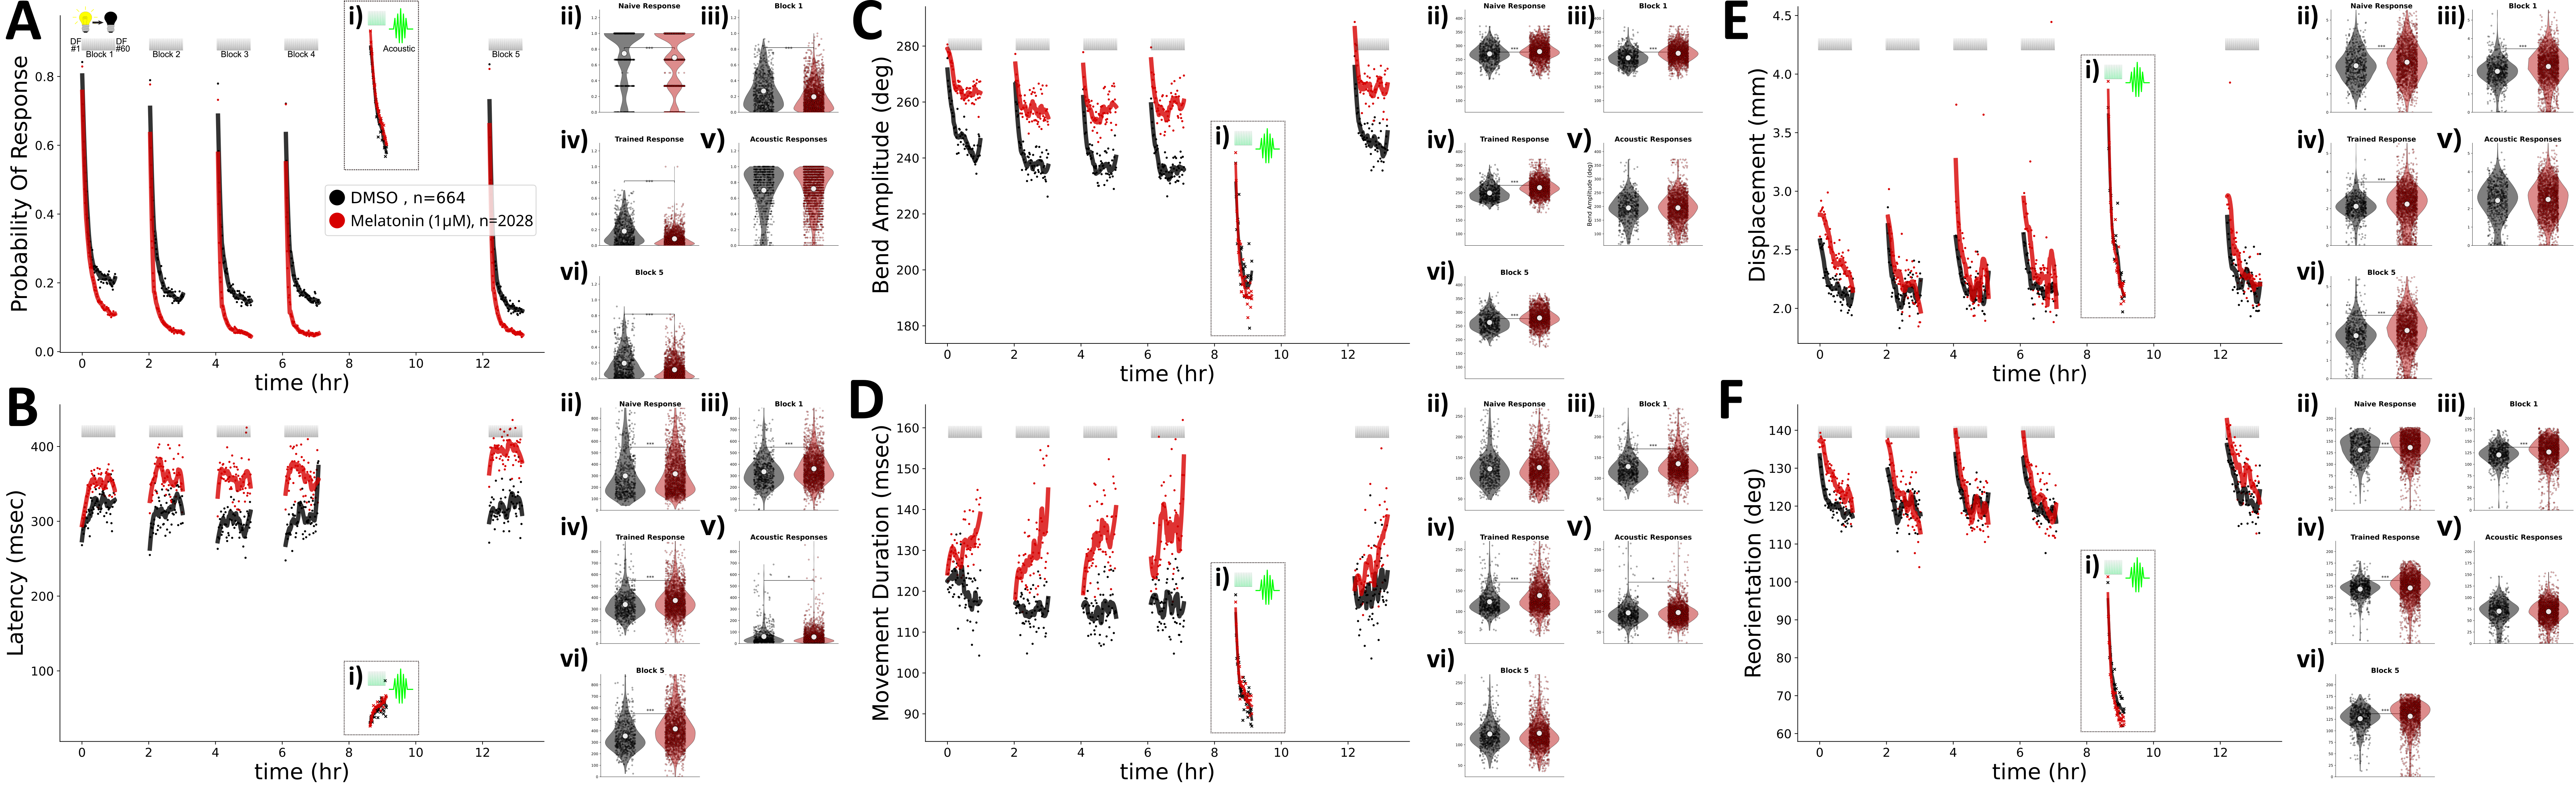
\includegraphics[width=1\linewidth]{Figures/Figure_MelatoninBehaviourPhenotype.png}

\caption{\textbf{\emph{atp1a3a} mutants display abnormal postures and swimming patterns}\\
\textbf{A)} \emph{atp1a3a} gene structure highlighting the location of the 8 bp deletion in exon 8 that leads to a premature stop codon in exon 9. DNA sequence of target site and predicted atp1a3a protein length in wildtype and mutant zebrafish. gRNA target sequence is underlined. Wildtype atp1a3a consists of 1023 amino acids; atp1a3a mutant protein consists of 272 amino acids identical to wildtype and 78 frameshifted amino acids, yielding a total protein length of 350 amino acids.\\
\textbf{B)} Comparison of \emph{atp1a3a} and \emph{atp1a3b} expression levels in \emph{atp1a3a} mutants. Expression was quantified using RT-qPCR and normalized to \emph{actb2} expression. Relative expression levels are normalized to expression levels in \emph{atp1a3a}\textsuperscript{+/+} larvae. Data are presented as means $\pm$ SEM. * $p < 0.05$; ** $p < 0.01$; *** $p < 0.001$.\\
\textbf{C)} Unbalanced postures and abnormal swimming patterns in \emph{atp1a3a} mutants, including corkscrew swimming, and\\
\textbf{D)} stable postures with the tail bent to one side.\\
\textbf{E)} Head-embedded behavioural setup for quantifying tail kinematics in response to visual stimuli. Based on pi\_tailtrack \citep{Randlett2023}\\
\textbf{F)} \emph{atp1a3a} mutants display:  \textbf{i)} Periods of normal swimming interspersed with \textbf{ii)} periods with the "bent tail" phenotype with a persistent bend to the left of the midline (dashed line) in this instance.\\
\textbf{G)} Tail tracking traces of 3 WT larvae showing normal bursts of swimming/tail flicks (blue), with few substantial or long-lasting deviations in the tail angle relative to the midline.\\
\textbf{H)} Tail tracking traces of 3 \emph{atp1a3a} mutant larvae showing very bursty swimming patterns with vigorous activity followed by periods of quiescence, and many periods of persistent tail bends reflected as large deviations in the Tail Angle.
}

\label{fig:1}

\end{center}
% \endinternallinenumbers
\end{figure}


\section{Materials and Methods}

\subsection{Animal husbandry and care}
All experiments were carried out using larval zebrafish between 5 and 6 days post-fertilization (dpf), maintained in E3 embryo medium supplemented with 0.02\% HEPES (pH 7.2) at a density of approximately 1 larva per mL.
Larvae were housed in 10 cm petri dishes under a 14:10 h light/dark cycle at a constant temperature of 28-29°C.
Zebrafish were bred and maintained at the SickKids Zebrafish CORE facility (Toronto, Canada) and the Animalerie Zebrafish Rockefeller (AZR, SFR Santé Lyon Est, Lyon).
All housing and experimental procedures were conducted in accordance with institutional and national regulations.
French facilities were approved by the French Ministry of Agriculture and the Ministry of Higher Education and Research (Agreement \#C693870602) and overseen by the local ethics committee (comité d’éthique en expérimentation animale de la Région Rhône-Alpes: CECCAPP).
Experiments conducted in Canada were approved by the University of Toronto Animal Care Committee, in accordance with guidelines established by the Canadian Council for Animal Care (CCAC).


\subsection{Generation of the \emph{atp1a3a} mutant line}
The \emph{atp1a3a} CRISPR mutant zebrafish line was generated at the SickKids Zebrafish CORE facility (Toronto, Canada).
The guide RNA (gRNA) was designed to target the \emph{atp1a3a} gene 82 base pairs downstream of the start of exon 8.
This specific region was chosen due to its close proximity to two human mutations known to cause Rapid-onset Dystonia Parkinsonism (821T>C mutation and 829G>A mutation).
The resultant \emph{atp1a3a} mutant allele has an 8 base pair deletion in exon 8 leading to a frameshift mutation with a premature stop in exon 9.
For Ca\textsuperscript{2+} imaging experiments, \emph{atp1a3a} mutants were crossed with \emph{Tg(elavl3:H2B-GCaMP6f); mitfa\textsubscript{-/-}}, to generate a line that express the nuclear-targeted GCaMP6f Ca2+ indicator pan-neuronally, in the pigment deficient \emph{Nacre} mutants.


\subsection{Genotyping}
Larvae were lysed in 50 mM NaOH at 95°C for 10 min and neutralized with 1 M Tris-HCl (pH 8.0) in a 1:9 volume ratio (Tris:NaOH), to extract genomic DNA.
Target region of atp1a3a was amplified using FIREPol® Master Mix Ready to Load 1× (Solis Biodyne) and gene-specific primers at 0.1 \textmu M.
Primer sequences used were: Forward : CGGTATTGTGGTCTGCACCG, Reverse: GCCGGTGATGATGTGGATGA.
Wild-type alleles yielded amplicons of 119 bp, while mutant alleles are 111 bp, which were distinguished on an 3.5\% agarose gel.




\subsection{Analyses of Spontaneous Behaviour}
The spontaneous behaviour of larvae was recorded using a high-speed imaging system adapted from BonZeb-based kinematic tracking \citep{Guilbeault2021}.
The setup included a Sentech STC-CMB200PCL CameraLink camera (Aegis Electronic Group, Inc.) with a zoom lens (Kowa), connected via a GrabLink Full XR Frame Grabber (Euresys Inc.) for acquisition of 1088 × 1088 resolution frames at 332 Hz.
Larvae were placed on a 6 mm thick transparent polycarbonate platform, illuminated from below by an 850 nm LED plate.
A 1920 × 1080, 60 Hz DLP pico projector (P7, AAXA Technologies Inc.) was integrated into the system, with projected light directed onto the platform using a cold mirror (Knight Optical).
Real-time video acquisition and processing were carried out in the Bonsai programming environment \citep{Lopes2015}, which interfaced with BonZeb for automated tracking \citep{Guilbeault2021}.
This configuration was used to obtain free-swimming recordings of \emph{atp1a3a} mutants, from which subsets of frames were extracted in FIJI and z-projected to generate composite images illustrating abnormal phenotypes and swim sequences.
Free swimming was further analyzed at 5 dpf using the 300-well plate setup we have previously described, where larvae are recorded in 8mm x 6mm (diameter x depth) wells \citep{Lamire2023-he}. 
Larvae were recorded over a 30-minute period in the absence of visual and acoustic stimulation.
From these recordings, the mean displacement per bout (mm), mean bout duration (s), mean peak bout speed (mm/s), total displacement (mm), and bout frequency (Hz) were calculated using custom python scripts (available at \href{https://github.com/owenrandlett/2025_atp1a3a}{github.com/owenrandlett/2025\_atp1a3a}).

\subsection{Analyses of the Optomotor Response (OMR)}

The OMR was assessed in 5dpf larvae in an acrylic arena containing 3 separate corridors allowing fish to swim in a 10.4cm x 2cm arena.
Larvae were subjected to alternating vertically moving OMR gratings using a projector (AAXA LED Pico Projector) and a 45° cold mirror.
OMR gratings were calcualted and dynamically displpayed using the “PsychoPy” package in python \citep{Peirce2007}
The gratings ran continually for 20 seconds epochs, alternating between directions along the long-axis of the arena, spanned by a 10 second long "no-stimulus" interval.
In total, the alternating OMR stimuli ran for 10 minutes, subjecting each larva to a total of 20 repeats of the stimuli.
Fish were tracked using IR LED arrays, and a camera (Chameleon 3 USB3 FLIR) running at 30 frames per second with an IR filter, and custom machine-vision scripts (available at \href{https://github.com/owenrandlett/2025_atp1a3a}{github.com/owenrandlett/2025\_atp1a3a}).
Lighting was projected at a screen under the arena using a projector (AAXA LED Pico Projector) and a 45° cold mirror.


\subsection{Analyses of the Dark Flash Response}
Larval behavior was assessed in custom 300-well acrylic plates (8 mm diameter, 6 mm depth; ~300 µL water volume) based on a modified version of previously described setups.
The plates were positioned beneath a 31\degree C water bath, which served as a heated lid to prevent condensation and maintain the wells at 29\degree C.
Recordings were captured using a Mikrotron CXP-4 camera (500 Hz) connected to a Silicon Software frame grabber (Marathon ACX-QP, Basler) and illuminated with IR LEDs (TSHF5410, digikey.com).
Visual stimulation was provided by a rectangular array of 155 WS2813 RGB LEDs, with dark flashes (DFs) consisting of a 1 second light-off period followed by a linear return to baseline over 20 seconds.
Acoustic/vibration taps were delivered via a solenoid (ROB-10391, Sparkfun).
The experimental design alternated 1 hour of stimulation with 1 hour of rest, during which a stepper motor-driven actuator (Hanpose HPV4, 500 cm) moved the camera between two plates, enabling up to 600 larvae to be tested simultaneously.

Control of the LEDs, solenoid, and camera actuator was managed by a Raspberry Pi Pico running CircuitPython and custom Python software, which also handled video acquisition and online tracking of head and tail positions at 20-30 Hz.
During DF or tap delivery, a 1 second high-speed burst recording was captured and later analyzed offline using background subtraction and morphological operations.
Tracking and analysis relied on open-source libraries, including OpenCV, scikit-image, NumPy, SciPy, and Numba.


\subsection{MAP-Mapping Analyses of Brain-Wide Activity Patterns}
Whole-brain activity mapping was performed using a MAP-mapping pipeline adapted from Randlett et al. (2015).
Cohorts of 150-200 larvae produced from adult atp1a3a+/- ; mitfa-/- ; Tg(elavl3:Huc-GCaMP6f) incross were subjected to visual stimuli as following:
For free swimming, larvae were grouped in one 10 cm petri dish and left swimming in a lit environment for 40 minutes in the same behavior setup as was used for the OMR stimulation (described below) to ensure identical external conditions.
For OMR stimulation, larvae were grouped in one 10 cm petri dish, left to acclimatize for 10 minutes then subjected to concentric gratings that alternated vertically each 30 seconds, using the OMR behavior setup.
For dark flash stimulation, larvae were grouped in one 10 cm petri dish, left to acclimatize for 20 minutes then subjected to 10 dark flashes following the dark flash protocol and using the dark flash habituation setup.
Larvae were then fixed and processed for immunohistochemistry with anti-pERK (Cell Signaling Technology, \#4370S) and anti-tERK primary antibodies (Cell Signaling Technology, \#4696S), followed by fluorophore-conjugated secondary antibodies: Alexa FluorTM 647 for tERK (Thermo Fisher Scientific, \#A21235) and Alexa FluorTM 568 for pERK (Thermo Fisher Scientific, \#11036).
Brains were imaged in dorsal orientation on the Leica Stellaris 5 confocal microscope equipped with a 25× water-immersion objective (HC FLUOTAR L 25x/0.95 W VISIR, CIQLE imaging platform, Lyon).
Image stacks were acquired at a voxel resolution of 0.08 × 0.08 × 2 µm, and two partially overlapping volumes were tiled to encompass the entire brain.
The GCaMP6f channel was used as an anatomical reference for nonlinear registration of each specimen to a standardized reference brain via the Computational Morphometry Toolkit (CMTK).
Registered image volumes were subsequently down-sampled to 300 × 679 × 80 voxels (x, y, z) and spatially smoothed using a two-dimensional Gaussian filter.
To account for inter-individual variability in staining intensity and morphology, voxel-wise pERK signals were normalized to corresponding tERK values prior to statistical comparison across experimental conditions.

\subsection{Calcium imaging and head-embedded behavioural analyses}



\subsection{Data analysis}
For the initial characterisation performed by Shahrzad, phenotypic distributions were visualized and analyzed using multiple statistical approaches.

Pie charts depicting the relative proportions of phenotypes in atp1a3a mutants were generated with Python packages Matplotlib, Pandas, and NumPy.

The same visualization pipeline was employed for phenotype transience assays, while histograms of tail angle distributions were constructed using these packages as well.

Statistical evaluation of swim kinematics during OMR assays was conducted with the Pingouin library.

Outliers were identified as values exceeding 1.5 times the interquartile range below the first quartile or above the third quartile and were excluded prior to subsequent analyses.

For RT-qPCR, relative expression levels of atp1a3a and atp1a3b were quantified using the $\Delta\Delta Ct$ method.

Data were analyzed with one-way ANOVAs followed by Bonferroni-corrected post hoc t-tests.

Outlier replicates were defined as those with |z| > 3.5 and removed prior to analysis.

A threshold of p < 0.05 was adopted to determine statistical significance in all tests.

Data analysis was carried out in Python using a custom-developed script.

Behavioral events were operationally defined based on cumulative tail bend angle thresholds, with deflections greater than 3 radians classified as O-bends and those exceeding 1 radian designated as C-bends.

The computational framework integrated several open-source libraries: NumPy, Pandas, Numba and SciPy for statistical procedures.

Data visualization was performed using Matplotlib and seaborn.

Statistical comparisons between distributions were conducted using the non-parametric Mann-Whitney U test as implemented in SciPy.



\section{Acknowledgments}

We are grateful to the staff of the PRECI and AZR zebrafish facilities, including Laure Benard, Robert Renard, Annie Desenfant, Olivier Lohez, for the expert care provided to the zebrafish. 
Imaging was performed in the CIQLE imaging platform (LYMIC, Lyon), and we thank the staff of the CIQLE for their support with confocal and 2-photon microscopy and image processing.
We also gratefully acknowledge the communities that develop and maintain the numerous open-source software packages we rely on, most of which could not be cited here.
HCR probes for \emph{npy}, \emph{penka}, \emph{penkb}, \emph{tac1} were a generous gift from Herwig Baier's laboratory.


\section{Funding}
This work was supported by funding from the ATIP-Avenir program of the CNRS and Inserm, a Fondation Fyssen research grant, and the IDEX-Impulsion initiative of the University of Lyon.

\bibliography{References_MtnRHab}

\newpage




\end{document}